\section{The \commonalities Approach}
\label{chap:improvement:commonalities}

\mnote{Approach overview}
We have motivated the idea of representing common concepts of redundantly or dependently represented elements of different metamodels in terms of \commonalities in explicit \conceptmetamodels rather than implicitly encoding them in direct consistency relations between the metamodels.
In the following, we discuss the specification of \conceptmetamodels and the notion of manifestation relations in more detail.
We also depict how further benefits can be generated by composing \conceptmetamodels in terms of defining a hierarchy of them.
We call this approach of defining and composing \conceptmetamodels of \commonalities the \emph{\commonalities approach}.
Essential for the central benefit of this approach, which is mitigation of trade-offs between quality properties of transformation networks, is the inherent possibility to achieve a specific kind of tree topology, which we derive from the approach before discussing different options for its operationalization.


\subsection{Concept Metamodels}

\mnote{Structure of metamodels}
The inherent benefits of the \commonalities approach are given by the definition of additional \conceptmetamodels, across which consistency relations are expressed, instead of defining consistency relations between the \concretemetamodels.
How these \conceptmetamodels and the manifestation relations between them and the \concretemetamodels look like is not that relevant.
Still, we discuss how elements can represented as \commonalities in a \conceptmetamodel and which situations instead of pure redundancies representing exactly the same information as in the manifestation can exist.

\begin{figure}
    \centering
    \newcommand{\vdistance}{12em}
\newcommand{\hdistance}{23em}
\newcommand{\innerhdistance}{7.6em}
\newcommand{\classwidth}{4.7em}
\newcommand{\labeldistance}{0.9em}
\newcommand{\mmborder}{0.9em}
\newcommand{\referenceshift}{0.9em}

\begin{tikzpicture}

\pgfdeclarelayer{bg}
\pgfsetlayers{bg,main}


% METACLASSES

\umlclassvarwidth{java_class}{}{Class}{
name\\
packageName
}{\classwidth}  

\umlclassvarwidth[, right=\innerhdistance of java_class.north, anchor=north]{java_field}{}{Field}{
name\\
}{\classwidth} 

\umlassociationfromto{([yshift=\referenceshift]java_field.west-|java_class.east) -- node[uml cardinality start, pos=0, above right] {$1$} node[uml cardinality end, pos=1, above left] {$*$} ([yshift=\referenceshift]java_field.west)}
\umlassociationfromto{([yshift=-\referenceshift]java_field.west) -- node[uml cardinality start, pos=0, above left] {$*$} node[uml role end, pos=1, below right] {type} node[uml cardinality end, pos=1, above right] {$1$} ([yshift=-\referenceshift]java_field.west-|java_class.east)}

\umlclassvarwidth[, below right=5em and \hdistance of java_class.north, anchor=north]{uml_class}{}{Class}{
name\\
}{\classwidth} 

\umlclassvarwidth[, left=\innerhdistance of uml_class.north, anchor=north]{uml_association}{}{Association}{
name\\
}{\classwidth}

\umlclassvarwidth[, above=5em of uml_class.north, anchor=north]{uml_package}{}{Package}{
name\\
}{\classwidth}

\umlassociationfromto{([yshift=\referenceshift]uml_association.east) -- node[uml cardinality start, pos=0, above right] {$*$} node[uml role end, pos=1, below left] {from} node[uml cardinality end, pos=1, above left] {$1$} ([yshift=\referenceshift]uml_class.west)}
\umlassociationfromto{([yshift=-\referenceshift]uml_association.east) -- node[uml cardinality start, pos=0, above right] {$*$} node[uml role end, pos=1, below left] {to} node[uml cardinality end, pos=1, above left] {$1$} ([yshift=-\referenceshift]uml_class.west)}
\umlassociationfromto{(uml_package.south) -- node[uml cardinality start, pos=0, below left] {$1$} node[uml role end, pos=1, above right] {classes} node[uml cardinality end, pos=1, above left] {$*$} (uml_class.north)}

\umlclassvarwidth[, above right=\vdistance and 0.5*\hdistance-0.5*\innerhdistance of java_class.north, anchor=north]{oo_class}{}{Class\vphantom{p}}{
name\\
}{\classwidth} 

\umlclassvarwidth[, below=5em of oo_class.north, anchor=north]{oo_association}{}{Association}{
name\\
}{\classwidth}

\umlclassvarwidth[, right=1.2*\innerhdistance of oo_class.north, anchor=north]{oo_package}{}{Package}{
name\\
}{\classwidth}

\umlassociationfromto{([xshift=-0.8*\referenceshift]oo_class.south) -- node[uml cardinality start, pos=0, below right] {$1$} node[uml role end, pos=0, below left] {from} node[uml cardinality end, pos=0, above right] {$*$} ([xshift=-0.8*\referenceshift]oo_association.north)}
\umlassociationfromto{([xshift=1.2*\referenceshift]oo_association.north) -- node[uml cardinality start, pos=0, above left] {$*$} node[uml role end, pos=1, below right] {to} node[uml cardinality end, pos=1, below left] {$1$} ([xshift=1.2*\referenceshift]oo_class.south)}
\umlassociationfromto{(oo_package.west) -- node[uml cardinality start, pos=0, below left] {$1$} node[uml role end, pos=1, above right] {classes} node[uml cardinality end, pos=1, below right] {$*$} (oo_class.east)}


% METAMODELS

\coordinate (java_label_coordinate) at ([yshift=\labeldistance]java_class.north west);
\node[mmlabel, anchor=west] (java_label) at (java_label_coordinate) {Java};

\coordinate (uml_label_coordinate) at ([yshift=\labeldistance]uml_package.north east);
\node[mmlabel, anchor=east] (java_label) at (uml_label_coordinate) {UML};

\coordinate (oo_label_coordinate) at ([yshift=\labeldistance]$(oo_class.north)!0.5!(oo_package.north)$);
\node[mmlabel, anchor=center] (oo_label) at (oo_label_coordinate) {Object-oriented Design};

\begin{pgfonlayer}{bg}
    \node[mmbg, fit=(java_class)(java_field)(java_label_coordinate), inner sep=\mmborder] (java) {};
    \node[mmbg, fit=(uml_class)(uml_package)(uml_association)(uml_label_coordinate), inner sep=\mmborder] (uml) {};
    \node[conceptmmbg, minimum width=11.5em, fit=(oo_class)(oo_association)(oo_package)(oo_label_coordinate), inner sep=\mmborder] (oo) {};
\end{pgfonlayer}


% CONSISTENCY RELATIONS

\draw[manifests relation] ([xshift=-0.48*\classwidth]oo_class.south) -- node[manifests relation, above, sloped] {\manifestslabel} (java_class);
\draw[manifests relation] ([xshift=0.48*\classwidth]oo_class.south) -- node[manifests relation, above, sloped] {\manifestslabel} (uml_class);
\draw[manifests relation] (oo_association) -- node[manifests relation, above, sloped] {\manifestslabel} (java_field);
\draw[manifests relation] (oo_association) -- node[manifests relation, above, sloped] {\manifestslabel} (uml_association);
\draw[manifests relation] (oo_package) -- node[manifests relation, above, sloped] {\manifestslabel} (uml_package);

\end{tikzpicture}

    \caption[Multiple \commonality example for object-oriented design]{\Conceptmetamodel for object-oriented design with a \texttt{Class}, an \texttt{Association} and a \texttt{Package} \commonality and its relations to the \concretemetamodels \gls{UML} and Java with a different representation of associations as fields and packages as attributes of classes in Java.}
    \label{fig:improvement:multiple_commonalities_example}
\end{figure}

\mnote{Representation of packages}
\autoref{fig:improvement:multiple_commonalities_example} depicts an extension of the example given in \autoref{fig:improvement:one_commonality_example}.
In addition to classes, it contains the representation of packages and associations.
A package is represented as a dedicated \metaclass in \gls{UML}, which references the classes contained in that package.
Java, however, does not have an explicit representation of packages, but encodes them into the package names specified within classes and, additionally, represents them in a folder structure in which the source code files of the classes are persisted.
A \conceptmetamodel used to preserve consistency between packages represented in \gls{UML} and Java must represent this information in any way such that changes in Java code can be propagated into a \gls{UML} model to preserve their consistency and vice versa.
To sketch an extreme, this could even be achieved with some string attribute in the \conceptmetamodel that encodes this information in such a unique way that the necessary information for both instances of the \concretemetamodels can be generated.
Actually, a \conceptmetamodel should represent such information in a reasonable structure, whose concrete characteristics have to be defined the transformation developer.
For packages, either the representation in Java as attributes of classes or the representation in \gls{UML} as a dedicated \metaclass can be chosen.
In the given example, we define packages in the \conceptmetamodel as explicit \metaclasses, as this makes the containment structure of classes in packages explicit.
In addition, in the complete \gls{UML} and Java metamodel packages are represented hierarchically, which is also easier to express as a relation between dedicated elements rather than their implicit encoding in the package names of classes.

\mnote{Representation of associations}
Associations in \gls{UML} are used to define that classes are related to each other.
Each association defines two classes, denoting from which class to which class the association is defined.
Java does not provide an explicit representation of associations, which usually results in their implicit representation as fields of the class from which the association is defined and having the type of the class to which it is defined.
In the example, we have chosen to represent an association explicitly in the \conceptmetamodel.
Fields can, in the complete Java and \gls{UML} metamodels, be related to further elements than associations, thus having this distinction within the \conceptmetamodel gives it more semantics.
In addition, we have chosen to have the class from which the association is defined reference the association instead having this reference in the opposite direction as in the \gls{UML} metamodel.
No matter whether or not this is beneficial, still all necessary information to keep Java fields and \gls{UML} associations consistent is represented by the \conceptmetamodel.
It shows that for the \conceptmetamodel even a representation that differs from all its manifestations can be chosen.

\mnote{General rule for \conceptmetamodels}
As mentioned before, the only requirement to a \conceptmetamodel is that it must be able to represent all information that is necessary for defining manifestation relations to the \concretemetamodels, such that they are able to preserve consistency according to some consistency relation between the \concretemetamodels.
A general, but rather informal rule, which has proven to be beneficial in the implementation of a case study for our evaluation, is to select among different representation options the semantically richest.
In the example, we have thus chosen to represent packages explicitly instead of implicitly encoding them in package names of classes.
This improves expressiveness of the \conceptmetamodel and makes its information easier to use for defining manifestation relations without interpreting implicitly encoded information in each of these relations.


\subsection{Composition of Concepts}

\mnote{Multiple \commonalities}
We have so far discussed the idea of defining an additional \conceptmetamodel to represent the common concepts of two or more \concretemetamodels.
For the depicted example for Java and \gls{UML}, it seems reasonable to define the group the common concepts in object-oriented design in such a metamodel.
In \autoref{fig:improvement:running_example}, we have also considered \gls{PCM} components and their consistency relations to classes in \gls{UML} and Java.
Although we could define a component \commonality for \gls{PCM} components and classes in \gls{UML} and Java, and consider this \commonality next to the class \commonality for classes in \gls{UML} and Java, we will likely not do so because of several drawbacks.
First, a component \commonality does, semantically, not fit into the discussed \conceptmetamodel for object-oriented design. Thus, the \conceptmetamodel would have to be considered broader, potentially only as a generic \conceptmetamodel.
Second, and more importantly, such a construction would introduce further redundancies, as the relation between classes in \gls{UML}and Java is expressed via two \commonalities, once the class \commonality and once the component \commonality.

\mnote{Monolithic \commonalities}
To solve the problem of a redundant specification of the relation between classes in \gls{UML} and Java via class and component \commonalities, we could combine these two \commonalities to a single one, representing all necessary common information.
If, however, further elements share information with classes and components, they also have to be merged into the same \commonality.
In the extreme case, this could result in only having one large \commonality that is able to represent all related information.
The manifestation relations would then have to make all kinds of distinctions based on the information given in such a \commonality.

\mnote{Exemplary \commonality hierarchy}
An intuitive solution for the example scenario is to not consider classes in \gls{UML} and Java as manifestations of a component \commonality, but to consider the class \commonality as a manifestation of the component \commonality.
Then the relation between classes in \gls{UML} and Java is still represented across one specific class \commonality, whereas the manifestation relation of the component \commonality only has to be defined for the concept of classes instead of their concrete manifestations.

\begin{figure}
    \centering
    \newcommand{\vdistance}{7em}
\newcommand{\hdistance}{13em}
\newcommand{\classwidth}{5.5em}
\newcommand{\labeldistance}{1em}
\newcommand{\labelshift}{0.3*\classwidth}
\newcommand{\mmborder}{1em}

\begin{tikzpicture}

\pgfdeclarelayer{bg}
\pgfsetlayers{bg,main}


% METACLASSES

\umlclassvarwidth{java_class}{}{Class}{
name\\
}{\classwidth}  

\umlclassvarwidth[, right=0.8*\hdistance of java_class.north, anchor=north]{uml_class}{}{Class}{
name\\
}{\classwidth} 

\umlclassvarwidth[, above right=\vdistance and 0.5*\hdistance of java_class.north, anchor=north]{oo_class}{}{Class\vphantom{p}}{
name\\
}{\classwidth} 

\umlclassvarwidth[, right=\hdistance of oo_class.north, anchor=north]{pcm_component}{}{Component}{
name\\
}{\classwidth} 

\umlclassvarwidth[, above right=\vdistance and 0.5*\hdistance of oo_class.north, anchor=north]{component_component}{}{Component}{
name\\
}{\classwidth}

% METAMODELS

\coordinate (java_label_coordinate) at ([yshift=\labeldistance]java_class.north west);
\node[mmlabel, anchor=west] (java_label) at (java_label_coordinate) {Java};

\coordinate (uml_label_coordinate) at ([yshift=\labeldistance]uml_class.north east);
\node[mmlabel, anchor=east] (uml_label) at (uml_label_coordinate) {\acrshort{UML}};

\coordinate (oo_label_coordinate) at ([xshift=-4*\labelshift,yshift=\labeldistance]oo_class.north);
\node[mmlabel, anchor=west, align=left] (oo_label) at ([xshift=-0.5em, yshift=-0.7em]oo_label_coordinate) {Object-oriented\\ Design};

\coordinate (pcm_label_coordinate) at ([yshift=\labeldistance]pcm_component.north east);
\node[mmlabel, anchor=east] (pcm_label) at (pcm_label_coordinate) {\acrshort{PCM}};

\coordinate (component_label_coordinate) at ([yshift=\labeldistance]component_component.north);
\node[mmlabel, anchor=center] (component_label) at (component_label_coordinate) {Component-based Design};

\begin{pgfonlayer}{bg}
    \node[mmbg, fit=(java_class)(java_label.west), inner sep=\mmborder] (java) {};
    \node[mmbg, fit=(uml_class)(uml_label.east), inner sep=\mmborder] (uml) {};
    \node[conceptmmbg, fit=(oo_class)(oo_label_coordinate), inner sep=\mmborder] (oo) {};
    \node[mmbg, fit=(pcm_component)(pcm_label.east), inner sep=\mmborder] (pcm) {};
    \node[conceptmmbg, fit=(component_component)(component_label.west)(component_label.east), inner sep=\mmborder] (component) {};
\end{pgfonlayer}


% CONSISTENCY RELATIONS

\draw[manifests relation] (oo_class) -- node[manifests relation, above, sloped] {\manifestslabel} (java_class);
\draw[manifests relation] (oo_class) -- node[manifests relation, above, sloped] {\manifestslabel} (uml_class);
\draw[manifests relation] (component_component) -- node[manifests relation, above, sloped] {\manifestslabel} (oo_class);
\draw[manifests relation] (component_component) -- node[manifests relation, above, sloped] {\manifestslabel} (pcm_component);

\end{tikzpicture}

    \caption[Hierarchic composition of \conceptmetamodels]{\Conceptmetamodels for component-based and object-oriented design and their manifestation relations between each other and to \concretemetamodels for the example introduced in \autoref{fig:improvement:running_example}. Adapted from \owncite[Fig.~3]{klare2019models}.}
    \label{fig:improvement:composed_commonalities_example}
\end{figure}

\mnote{Hierarchic composition of \commonalities}
Abstracting from this concrete example, we propose to define hierarchies of \commonalities and \conceptmetamodels, such that a manifestation of a \commonality must not necessarily be some classes of a \concretemetamodel, but can also be \commonalities of other \conceptmetamodels.
We depict such a structure for the example of classes and components in \autoref{fig:improvement:composed_commonalities_example}.
This allows to define one \conceptmetamodel for each kind of concept, such as object-oriented design or component-based design, and then compose these concepts hierarchically.
In consequence, this avoids the specification of a single \conceptmetamodel that may be become unmanageably large and again suffers from bad modularity as it needs combine information from as many \concretemetamodels as are supposed to be kept consistent.

\mnote{Restriction to tree topology}
Since constructing such hierarchies induces a tree topology between the concrete and \conceptmetamodels, this construction suffers from the drawbacks regarding completeness, which we have already discussed in \autoref{chap:classification:topologies:effects}.
Given two concrete or \conceptmetamodels, there must be one that can be considered the manifestation of the other, or it must be possible to define a \conceptmetamodel for them, such that finally a tree of concrete and \conceptmetamodels is achieved.
First, this is actually an assumption and thus limitation of the approach, for which we provide preliminary results regarding applicability in our evaluation in \autoref{chap:commonalities_evaluation}.
Second, we further discuss these requirements regarding a tree structure in the following subsection to relax the restriction currently defined at the level of metamodels and consider a more fine-grained restriction at the level of \metaclasses.


\subsection{Tree Topology}

\mnote{Correctness guarantee}
In \autoref{chap:classification:topologies:effects}, we have discussed the benefits of a tree topology induced by the metamodels and transformations of a transformation network, especially concerning inherent correctness.
We have proposed the hierarchic composition of \conceptmetamodels in the previous subsection to achieve a tree structure of manifestation relations in the \commonalities approach, which leads to a transformation network having a tree topology when realizing the manifestation relations as transformations.

\begin{figure}
    \centering
    \newcommand{\vdistance}{7em}
\newcommand{\hdistance}{13em}
\newcommand{\classwidth}{5.5em}
\newcommand{\smallclasswidth}{4em}
\newcommand{\labeldistance}{1.0em}
\newcommand{\labelshift}{0.3*\classwidth}
\newcommand{\mmborder}{1em}


\begin{tikzpicture}

\pgfdeclarelayer{bg}
\pgfsetlayers{bg,main}


% METACLASSES

\umlclassvarwidth{java_class}{}{Class\vphantom{p}}{
name\\
}{\smallclasswidth}  

\umlclassvarwidth[, right=0.65*\hdistance of java_class.north, anchor=north]{uml_class}{}{Class\vphantom{p}}{
name\\
}{\smallclasswidth}

\umlclassvarwidth[, right=1.3*\classwidth of uml_class.north, anchor=north]{uml_component}{}{Component}{
name\\
}{\classwidth} 

\umlclassvarwidth[, above right=\vdistance and 0.5*\hdistance of java_class.north, anchor=north]{oo_class}{}{Class\vphantom{p}}{
name\\
}{\classwidth} 

\umlclassvarwidth[, right=\hdistance of oo_class.north, anchor=north]{pcm_component}{}{Component}{
name\\
}{\classwidth} 

\umlclassvarwidth[, above right=\vdistance and 0.5*\hdistance of oo_class.north, anchor=north]{component_component}{}{Component}{
name\\
}{\classwidth}

% METAMODELS

\coordinate (java_label_coordinate) at ([yshift=\labeldistance]java_class.north west);
\node[mmlabel, anchor=west] (java_label) at (java_label_coordinate) {Java};

\coordinate (uml_label_coordinate) at ([yshift=\labeldistance]uml_component.north east);
\node[mmlabel, anchor=east] (uml_label) at (uml_label_coordinate) {\acrshort{UML}};

\coordinate (oo_label_coordinate) at ([xshift=-4*\labelshift,yshift=\labeldistance]oo_class.north);
\node[mmlabel, anchor=west, align=left] (oo_label) at ([xshift=-0.5em, yshift=-0.7em]oo_label_coordinate) {Object-oriented\\ Design};

\coordinate (pcm_label_coordinate) at ([yshift=\labeldistance]pcm_component.north east);
\node[mmlabel, anchor=east] (pcm_label) at (pcm_label_coordinate) {\acrshort{PCM}};

\coordinate (component_label_coordinate) at ([yshift=\labeldistance]component_component.north);
\node[mmlabel, anchor=center] (component_label) at (component_label_coordinate) {Component-based Design};

\begin{pgfonlayer}{bg}
    \node[mmbg, fit=(java_class)(java_label.west), inner sep=\mmborder] (java) {};
    \node[mmbg, fit=(uml_class)(uml_component)(uml_label.east), inner sep=\mmborder] (uml) {};
    \node[conceptmmbg, fit=(oo_class)(oo_label_coordinate), inner sep=\mmborder] (oo) {};
    \node[mmbg, fit=(pcm_component)(pcm_label.east), inner sep=\mmborder] (pcm) {};
    \node[conceptmmbg, fit=(component_component)(component_label.west)(component_label.east), inner sep=\mmborder] (component) {};
\end{pgfonlayer}

\draw[-, color=gray] ($(uml_class.south east)!0.5!(uml_component.south west)-(0,\mmborder)$) -- ($(uml_class.north east)!0.5!(uml_component.north west)+(0,\mmborder+\labeldistance)$);


% CONSISTENCY RELATIONS

\draw[manifests relation] (oo_class) -- node[stereotype, above, sloped] {\manifestslabel} (java_class);
\draw[manifests relation] (oo_class) -- node[stereotype, above, sloped] {\manifestslabel} (uml_class);
\draw[manifests relation] (component_component) -- node[stereotype, above, sloped] {\manifestslabel} (oo_class);
\draw[manifests relation] (component_component) -- node[stereotype, above, sloped] {\manifestslabel} (pcm_component);
\draw[manifests relation] (component_component) -- node[stereotype, below, sloped] {\manifestslabel} ([xshift=-1.5em]uml_component.north);

\end{tikzpicture}

    \caption[Example for tree topology of \commonalities]{\Conceptmetamodels for component-based and object-oriented design and their manifestation relations between each other and to \concretemetamodels for the example introduced in \autoref{fig:improvement:running_example} and extended by components in \gls{UML}. Adapted from \owncite[Fig.~3]{klare2019models}.}
    \label{fig:improvement:extended_composed_commonalities_example}
\end{figure}

\mnote{Impracticality of trees}
That approach does, however, assume that such a tree topology of \conceptmetamodels can always be achieved.
Since we have up to now discussed the topology at the level of complete metamodels and transformations between them, it is easy to see that a tree cannot be achieved in many situations.
This is always the case if one \concretemetamodel contains concepts that are to be represented in multiple \conceptmetamodels.
For example, the \gls{UML} contains concepts both from object-oriented design and component-based design, which easily conflicts with the goal of achieving a tree topology.
\autoref{fig:improvement:extended_composed_commonalities_example} depicts this example for classes and components in \gls{UML}.
\gls{UML} classes have a common concept with the \concretemetamodels Java in object-oriented design and \gls{UML} components have a common concept with the \concretemetamodel \gls{PCM} in component-based design, which both, in turn, share a manifestation relation. This breaks the tree topology at the level of metamodels and transformations between them.

\mnote{Metamodel bounds}
Although the bounds of metamodels are usually motivated by their necessity to fit for a specific purpose (cf.\ \autoref{chap:foundations:modeling:models}) and thus to represent specific concepts, metamodels bounds are, in general, arbitrary.
Especially if metamodels have a rather general purpose, such as \gls{UML} or programming languages like Java, they may contains elements representing multiple different concepts or the same elements may even be considered manifestations of multiple concepts.
The former case leads to the situation that the elements of a metamodel may be separated by the different concepts they represent, thus virtually forming multiple metamodels.
Usually, however, even elements representing concepts from different domains are still related, for example, by having the same super types like \texttt{NamedElement}, which makes their separation into different metamodels impossible.

\mnote{Non-interference as relaxed notion}
The benefit of inherent correctness guarantees of transformation networks with tree topology arises from the fact that there are no two paths of transformations between the same metamodels, as discussed in \autoref{chap:classification:properties}.
This is, however, already given if two paths of transformations affect disjoint sets of elements and thus do not interfere.
Such a notion of \emph{non-interference} has already been defined by \textcite{stevens2020BidirectionalTransformationLarge-SoSym}, which defines that two transformations changing the same model do not interfere if changing their execution order does not change the result.
In consequence, since each transformation ensures consistency to its consistency relations and since the result is independent from the execution order of such non-interfering transformations, it is guaranteed that the resulting models are consistent to both non-interfering transformations.

\mnote{Consistency relation trees}
This informally stated notion of having all pairs of paths of transformations affect disjoint sets of elements, given, for example, by non-interference, conforms to our notion of \emph{consistency relation trees} as specified in \autoref{def:relationtree} for proving compatibility of consistency relations.
It defines that for each pair of concatenations of consistency relations either the left class tuples or the right class tuples must be disjoint, such that sequences of transformations preserving consistency to these relations affect disjoint sets of objects.
In consequence, it is sufficient to ensure that the graph of consistency relations defined by the manifestation relations is a consistency relation tree to ensure compatibility of the network.
Due to the lack of multiple transformation paths affecting the same elements, it is also not necessary to ensure that transformations are synchronizing.
Thus, even for this relaxed notion in comparison to trees at the level of metamodels and transformations, as depicted in \autoref{chap:classification:topologies:effects}, correctness guarantees for the transformation network are given.

\mnote{Practicality of relaxed notion}
Still, this relaxed notion represents a requirement for the \commonalities approach to provide specific benefits.
We show at a case study in our evaluation in \autoref{chap:commonalities_evaluation} that it is actually possible to achieve such a structure in practical scenarios, which serves as an indicator for its general achievability and thus the possibility to have inherent correctness guarantees when applying the \commonalities approach for preserving consistency of multiple models.

% NOTE: Hierarchy of commonalities still relevant, because only between concept metamodels manifestation relations are allowed


\subsection{Operationalization}
\label{chap:improvement:commonalities:operationalization}

\mnote{Deriving executable transformations}
Up to now, we have discussed how to express consistency by means of \conceptmetamodels with \commonalities and manifestation relations in the \commonalities approach.
To actually preserve consistency of instances of the \concretemetamodels, such a specification must also be operationalized, such that executable transformations that can be applied after changes to these models are present or derived.

\begin{figure}
    \centering
    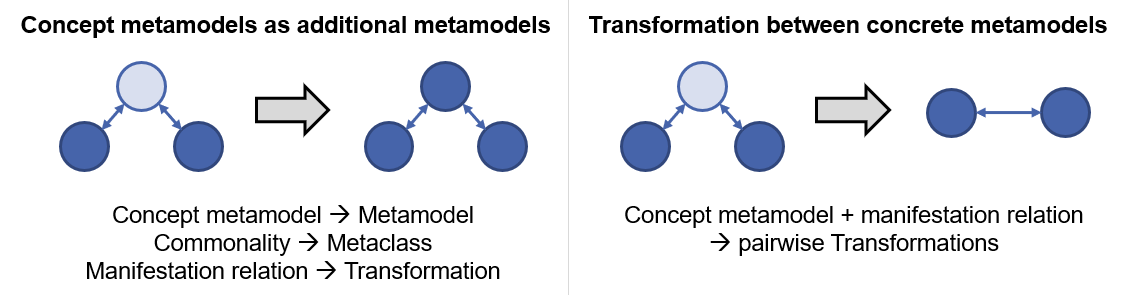
\includegraphics[width=\textwidth]{figures/quality/improvement/operationalization_alternatives.png}
    \caption[Alternatives for \commonalities operationalization]{Exemplification of alternatives to operationalize \commonalities specifications by using \conceptmetamodels as ordinary metamodels or by deriving direct transformations from them.}
    \label{fig:improvement:operationalization_alternatives}
\end{figure}

\mnote{Operationalization options}
We can distinguish two basic options how to operationalize a specification of \commonalities, which are also depicted in \autoref{fig:improvement:operationalization_alternatives}:
\begin{properdescription}
    \item[\Conceptmetamodels as additional metamodels:] \Conceptmetamodels are considered as ordinary metamodels and manifestation relations are considered as ordinary transformations, thus we consider a transformation network of \concretemetamodels and \conceptmetamodels, whose instances are kept consistent by transformations realizing their manifestation relations. In consequence, instances of the \conceptmetamodels have to be maintained.
    \item[Transformations between \concretemetamodels:] \Conceptmetamodels and the manifestation relations are only used as auxiliary specification artifacts, from which direct transformations between the \concretemetamodels are derived. For example, from the \conceptmetamodel for object-oriented design in \autoref{fig:improvement:one_commonality_example}, a transformation between Java and \gls{UML} is derived.
\end{properdescription}

\mnote{\Conceptmetamodels as ordinary metamodels}
The benefits of treating \conceptmetamodels as ordinary, additional metamodels and the manifestation relations as transformations is easy achievability.
No specific languages or generators are required to derive the required artifacts, but existing tools for defining metamodels and transformations can be used to define \conceptmetamodels and manifestation relations that can be readily used to preserve consistency of their instances.
A drawback of this approach is that it requires the management and persistence of additional artifacts, namely the instances of the \conceptmetamodels, which are only auxiliary artifacts that should be transparent to the user.
This can, however, be hidden by an according framework that abstracts from these additional artifacts, such that developers are still only confronted with the models of the tools they use.
Such functionality is provided by tools like \vitruv~\cite{klare2020Vitruv-JSS}.

\mnote{Deriving direct transformations}
Deriving transformations between \concretemetamodels from a specification of \conceptmetamodels and manifestation relations benefits from not introducing further artifacts, such that a developer still only has to deal with instances of the \concretemetamodels he or she is concerned with.
This approach, however, suffers from reduced expressiveness, because not all multiary relations as expressed across additional \conceptmetamodels (cf.~\cite{diskin2018MultiModelSynchronization-FASE}) can be expressed by sets of binary relations and transformations preserving them (cf.~\cite{stevens2020BidirectionalTransformationLarge-SoSym}).
In addition, it requires the implementation of generators that derive transformations from specification of \conceptmetamodels and manifestation relations.

\mnote{Correctness of derived transformation network}
Although with the second approach of deriving ordinary transformations the resulting transformation network contains cycles and does thus not provide the benefit of correctness guarantees due to its topology, it still provides this guarantee, because the transformations were generated from a specification that ensures correctness.
For example, since the specification with \commonalities cannot contains any incompatibilities, the transformations derived from them cannot contain them either, as long as the generator produces transformations that actually preserve consistency conforming to the defined manifestation relations.

\mnote{Multiple transformation executions}
For the orchestration of the generated transformations, no matter whether they are defined to \conceptmetamodels or derived between the \concretemetamodels, it is still necessary to allow the execution of each transformation multiple times.
Due to the situations identified in \autoref{chap:orchestration}, in which it is necessary to execute transformations multiple times to \enquote{negotiate} a result and repeatedly react to the changes of other transformations, such a behavior is still relevant for the \commonalities approach.
For example, propagating a class from Java across the object-oriented design \conceptmetamodels and the component-based design \conceptmetamodel to a component in \gls{PCM} can lead to further additions to the class as soon as its identified as representation of component, which then needs to be propagated back to the class representation in Java.
Transformations are still synchronizing and thus allowed to modify both involved models to support such situations, which can make this backpropagation of changes necessary.


% \begin{copiedFrom}{DocSym} % ABOUT TREES

% The most crucial part of this approach is the necessity to build a tree of \glspl{CMM}.
% This will not be possible if always considering whole metamodels and their relations, but can be possible if independent concepts are extracted to be treated individually.
% %For that, we will apply our findings on consistency relation decomposition (see \autoref{chap:improvement:approach}).
% %This is similar to decomposing consistency relations, as introduced in \autoref{sec:approach:decomposition}, which is why we will apply our findings therefrom.
% Additionally, the approach specifically aims to improve the specification of transformations for descriptive relations.
% In consequence, it must be combined with transformations expressing the normative relations between \glspl{CMM} and other metamodels.

% \end{copiedFrom} % DocSym

% \begin{copiedFrom}{VoSE}

% The state-of-the-art approach to keep models consistent automatically is the application of transformation languages.
% If instances of multiple (i.e., more than two) metamodels are to be kept consistent, one can either use multidirectional transformation approaches, or compose bidirectional transformations to a network of transformations~\cite{cleve2019dagstuhl}.
% Following sentence moved to introduction
%Such a network can be regarded as a graph, formed by metamodels as its nodes and transformations as its edges.
% When an instance of one metamodel is changed in such a network, the transformations are executed successively to propagate the change transitively across all models.
% There are strategies to find one ordering of transformations to apply~\cite{stevens2020BidirectionalTransformationLarge-SoSym} and strategies to perform a fixpoint iteration until no further changes are conducted~\cite{klare2019icmt}.

% %Short introduction of transformation network, what nodes and edges are and so on.
% In this section, we propose a different approach for keeping two or more models consistent by specifying their common concepts rather than their direct consistency relations.
% This forms our contribution~\autoref{contrib:quality:improvement}.
% % \subsection{Defining Consistency Relations}
% % Different metamodels provide

% Consistency relations are usually defined declaratively (what constraints have to hold) or imperatively (how are constraints enforced) between two (or sometimes more) metamodels.
% This is a definition of when instances of that metamodels are considered consistent.
% Consistency constraints can be either \emph{declarative} or \emph{normative}. Declarative constraints exist (e.g. because they are somehow \enquote{natural} and have to be formalized to be checked or preserved by a tools. Normative constraints do not have to adhere to an existing notion of consistency and thus implicitly define what is considered consistent.
% In our running example, the constraints between UML and Java exist and only have to be specified in a declarative manner.
% On the other hand, the constraints between architecture and OO design (i.e. PCM and UML/Java) were normatively defined by \textcite{langhammerconstraints}. There is no single correct mapping between architecture and OO design but several possible.

% \subsection*{Composing \commonalities}

% We have explained how multiple metamodels can be kept consistent using one \conceptmetamodel.
% This allows, theoretically, the definition of one large \conceptmetamodel that contains all \commonalities for all \concretemetamodels.
% It would at first sight be similar to a \gls{SUMM}, as introduced by \textcite{atkinson2010a}.
% However, it would be less complex than a \gls{SUMM}, which is able to express all information about the software system and thus contains the union of all \concretemetamodels.
% %In fact, the resulting \conceptmetamodel would be comparable to a \summ according to \textcite{atkinson2010a}, which is able to express all information about the software system, whereas the instances of the \concretemetamodels would only serve as projectional views that do not provide further information.
% Nevertheless, one large \conceptmetamodel would still become unmanageably large due to the fact that it had to contain the union of all pairwise intersections of the \concretemetamodels, as mentioned before.

% \begin{figure}
%     \centering
%     \newcommand{\vdistance}{7.5em}
\newcommand{\hdistance}{11em}
\newcommand{\classwidth}{5.5em}
\newcommand{\labeldistance}{1.2em}
\newcommand{\labelshift}{0.3*\classwidth}
\newcommand{\representstext}{\emph{«manifests»}}
\newcommand{\mmborder}{0.9em}

\begin{tikzpicture}

\pgfdeclarelayer{bg}
\pgfsetlayers{bg,main}


% METACLASSES

\umlclassvarwidth{java_class}{}{Class}{
name\\
}{\classwidth}  

\umlclassvarwidth[, right=\hdistance of java_class.north, anchor=north]{uml_class}{}{Class}{
name\\
}{\classwidth} 

\umlclassvarwidth[, above right=\vdistance and 0.5*\hdistance of java_class.north, anchor=north]{oo_class}{}{Class\vphantom{p}}{
name\\
}{\classwidth} 

\umlclassvarwidth[, right=\hdistance of oo_class.north, anchor=north]{pcm_component}{}{Component}{
name\\
}{\classwidth} 

\umlclassvarwidth[, above right=\vdistance and 0.5*\hdistance of oo_class.north, anchor=north]{component_component}{}{Component}{
name\\
}{\classwidth}

% METAMODELS

\coordinate (java_label_coordinate) at ([xshift=-\labelshift,yshift=\labeldistance]java_class.north);
\node[mmlabel, anchor=center] (java_label) at (java_label_coordinate) {Java};

\coordinate (uml_label_coordinate) at ([xshift=\labelshift,yshift=\labeldistance]uml_class.north);
\node[mmlabel, anchor=center] (java_label) at (uml_label_coordinate) {UML};

\coordinate (oo_label_coordinate) at ([xshift=-4*\labelshift,yshift=\labeldistance]oo_class.north);
\node[mmlabel, anchor=west, align=left] (oo_label) at ([xshift=-0.7em, yshift=-0.8em]oo_label_coordinate) {Object-oriented\\ Design};

\coordinate (pcm_label_coordinate) at ([xshift=\labelshift,yshift=\labeldistance]pcm_component.north);
\node[mmlabel, anchor=center] (pcm_label) at (pcm_label_coordinate) {PCM};

\coordinate (component_label_coordinate) at ([yshift=\labeldistance]component_component.north);
\node[mmlabel, anchor=center] (component_label) at (component_label_coordinate) {Componend-based Design};

\begin{pgfonlayer}{bg}
    \node[mmbg, fit=(java_class)(java_label_coordinate), inner sep=\mmborder] (java) {};
    \node[mmbg, fit=(uml_class)(uml_label_coordinate), inner sep=\mmborder] (uml) {};
    \node[conceptmmbg, fit=(oo_class)(oo_label_coordinate), inner sep=\mmborder] (oo) {};
    \node[mmbg, fit=(pcm_component)(pcm_label_coordinate), inner sep=\mmborder] (pcm) {};
    \node[conceptmmbg, minimum width=12.5em, fit=(component_component)(component_label_coordinate), inner sep=\mmborder] (component) {};
\end{pgfonlayer}


% CONSISTENCY RELATIONS

\draw[directed consistency relation] (oo_class) -- node[above, sloped] {\representstext} (java_class);
\draw[directed consistency relation] (oo_class) -- node[above, sloped] {\representstext} (uml_class);
\draw[directed consistency relation] (component_component) -- node[above, sloped] {\representstext} (oo_class);
\draw[directed consistency relation] (component_component) -- node[above, sloped] {\representstext} (pcm_component);

\end{tikzpicture}

%     \caption[Concept metamodels for the running example]{\Conceptmetamodels (dark) and their relations to \concretemetamodels (light) for the running example.}
%     \label{fig:quality:composed_commonalities_example}
% \end{figure}

% To avoid the specification of such a monolithic \conceptmetamodel, we propose to compose \commonalities from different \conceptmetamodels.
% Instead of having only \commonalities that relate to \metaclasses in \concretemetamodels, \commonalities may also have relations to other \commonalities.
% Consider the \conceptmetamodel for component-based design in \autoref{fig:quality:composed_commonalities_example}.
% It contains the \commonality \texttt{Component}, which is represented by an equally named \metaclass in \gls{PCM},
% as well as in the \commonality \texttt{Class} in the \conceptmetamodel for object-oriented design, conforming to the relations proposed by \textcite{langhammer2015a}.
% This induces a tree structure with \commonalities as inner nodes and \metaclasses of \concretemetamodels as leaves.
% With such a composition structure, a \emph{«manifests»} relation may not only exist between a %concrete and a concept metamodel but also between two \conceptmetamodels.
% \commonality of a \conceptmetamodel and a \metaclass in a \concretemetamodel but also between two \commonalities.
% However, a concrete or \conceptmetamodel that is lower in the hierarchy is supposed to represent how a \metaclass or \commonality in the higher one manifests, which is why we call it a \emph{manifestation}.
% %Due to that, we call concrete and \conceptmetamodels that contain \metaclasses or \commonalities with a \emph{«manifests»} relation to another \conceptmetamodel a \emph{manifestation} of that \conceptmetamodel.
% For example, the object-oriented design \conceptmetamodel is a manifestation of the component-based design \conceptmetamodel.

% \begin{figure}
%     \centering
%     \newcommand{\vdistance}{8em}
\newcommand{\hdistance}{11.5em}
\newcommand{\classwidth}{5.5em}
\newcommand{\smallclasswidth}{4em}
\newcommand{\labeldistance}{1.2em}
\newcommand{\labelshift}{0.3*\classwidth}
\newcommand{\representstext}{\emph{«manifests»}}
\newcommand{\mmborder}{1em}

\begin{tikzpicture}

\pgfdeclarelayer{bg}
\pgfsetlayers{bg,main}


% METACLASSES

\umlclassvarwidth{java_class}{}{Class\vphantom{p}}{
name\\
}{\smallclasswidth}  

\umlclassvarwidth[, right=0.65*\hdistance of java_class.north, anchor=north]{uml_class}{}{Class\vphantom{p}}{
name\\
}{\smallclasswidth}

\umlclassvarwidth[, right=1.3*\classwidth of uml_class.north, anchor=north]{uml_component}{}{Component}{
name\\
}{\classwidth} 

\umlclassvarwidth[, above right=\vdistance and 0.5*\hdistance of java_class.north, anchor=north]{oo_class}{}{Class\vphantom{p}}{
name\\
}{\classwidth} 

\umlclassvarwidth[, right=\hdistance of oo_class.north, anchor=north]{pcm_component}{}{Component}{
name\\
}{\classwidth} 

\umlclassvarwidth[, above right=\vdistance and 0.5*\hdistance of oo_class.north, anchor=north]{component_component}{}{Component}{
name\\
}{\classwidth}

% METAMODELS

\coordinate (java_label_coordinate) at ([xshift=-\labelshift,yshift=\labeldistance]java_class.north);
\node[mmlabel, anchor=center] (java_label) at (java_label_coordinate) {Java};

\coordinate (uml_label_coordinate) at ([xshift=\labelshift,yshift=\labeldistance]uml_component.north);
\node[mmlabel, anchor=center] (java_label) at (uml_label_coordinate) {UML};

\coordinate (oo_label_coordinate) at ([xshift=-4*\labelshift,yshift=\labeldistance]oo_class.north);
\node[mmlabel, anchor=west, align=left] (oo_label) at ([xshift=-0.7em, yshift=-0.8em]oo_label_coordinate) {Object-oriented\\ Design};

\coordinate (pcm_label_coordinate) at ([xshift=\labelshift,yshift=\labeldistance]pcm_component.north);
\node[mmlabel, anchor=center] (pcm_label) at (pcm_label_coordinate) {PCM};

\coordinate (component_label_coordinate) at ([yshift=\labeldistance]component_component.north);
\node[mmlabel, anchor=center] (component_label) at (component_label_coordinate) {Componend-based Design};

\begin{pgfonlayer}{bg}
    \node[mmbg, fit=(java_class)(java_label_coordinate), inner sep=\mmborder] (java) {};
    \node[mmbg, fit=(uml_class)(uml_component)(uml_label_coordinate), inner sep=\mmborder] (uml) {};
    \node[conceptmmbg, fit=(oo_class)(oo_label_coordinate), inner sep=\mmborder] (oo) {};
    \node[mmbg, fit=(pcm_component)(pcm_label_coordinate), inner sep=\mmborder] (pcm) {};
    \node[conceptmmbg, minimum width=12.5em, fit=(component_component)(component_label_coordinate), inner sep=\mmborder] (component) {};
\end{pgfonlayer}

\draw[-, color=gray] ($(uml_class.south east)!0.5!(uml_component.south west)-(0,\mmborder)$) -- ($(uml_class.north east)!0.5!(uml_component.north west)+(0,\mmborder+\labeldistance)$);


% CONSISTENCY RELATIONS

\draw[consistencyrel, <-] (java_class) -- node[above, sloped] {\representstext} (oo_class);
\draw[consistencyrel, <-] (uml_class) -- node[above, sloped] {\representstext} (oo_class);
\draw[consistencyrel, <-] (oo_class) -- node[above, sloped] {\representstext} (component_component);
\draw[consistencyrel, <-] (pcm_component) -- node[above, sloped] {\representstext} (component_component);
\draw[consistencyrel, <-] ([xshift=-1.5em]uml_component.north) -- node[below, sloped] {\representstext} (component_component);

\end{tikzpicture}

%     \caption[Concept metamodels in the running example]{\Conceptmetamodels (dark) and \concretemetamodels (light) of the running example, extended by UML components, with their relations.}
%     \label{fig:quality:extended_composed_commonalities_example}
% \end{figure}

% Our goal is to achieve a tree structure of commonalities. In the extended example in \autoref{fig:quality:extended_composed_commonalities_example}, a \texttt{Component} in the \conceptmetamodel for component-based design does not only manifest in a \gls{PCM} \texttt{Component} as well as a \texttt{Class} in object-oriented design, but also in \gls{UML}.
% Since a \texttt{Class} in object-oriented design manifests both in Java and \gls{UML}, we do not have a tree structure of the induced relations between the metamodels anymore, due to \texttt{Class} and \texttt{Component} both being represented in \gls{UML}.
% However, This still induces a tree structure between \metaclasses and \commonalities, with the \commonalities being inner nodes and \metaclasses of \concretemetamodels being leaves.

%
% How are Commonalities composed to keep multiple models consistent? What about overlaps?
% Apply to OO and PCM case
%
% \begin{figure}
%     \centering
% %    \includegraphics[width=\columnwidth]{figures/dag_example.pdf}\\
%     \newcommand{\vdistance}{4.8em}
\newcommand{\hdistance}{10.9em}
\newcommand{\mmwidth}{8.5em}
\newcommand{\mmheight}{3em}

\begin{tikzpicture}[
    mm/.style={draw, mmbg, minimum width=\mmwidth, minimum height=\mmheight, inner sep=0em}, %, font=\itshape},
    conceptmm/.style={mm, conceptmmbg},
]

% Metamodels

\node[mm] (java) {Java};
\node[mm, draw=gray!70, minimum height=0.5*\mmheight, right=\hdistance of java.south, anchor=south] (uml) {UML};
\node[mm, draw=gray!70, minimum width=0.5*\mmwidth, minimum height=0.5*\mmheight, above=0.5*\mmheight of uml.west, anchor=west] (uml_class) {\emph{Class}};
\node[mm, draw=gray!70, minimum width=0.5*\mmwidth, minimum height=0.5*\mmheight, above=0.5*\mmheight of uml.east, anchor=east] (uml_component) {\emph{Comp}};
\node[mm, fill=none, right=\hdistance of java.north, anchor=north] {}; % Redraw thick border of UML
\node[conceptmm, above right=\vdistance and 0.5*\hdistance of java.north, anchor=north, align=center] (oo) {Object-oriented\\ Design};
\node[mm, right=\hdistance of oo.north, anchor=north] (pcm) {PCM};
\node[conceptmm, above right=\vdistance and 0.5*\hdistance of oo.north, anchor=north, align=center] (component) {Component-based\\ Design};


% CONSISTENCY RELATIONS

\draw[consistencyrel, <-] (java) -- (oo);
\draw[consistencyrel, <-] (uml_class) -- (oo);
\draw[consistencyrel, <-] (oo) -- (component);
\draw[consistencyrel, <-] ([xshift=-0.15*\mmwidth]uml_component.north) -- (component);
\draw[consistencyrel, <-] (pcm) -- (component);


\end{tikzpicture}
 %\\[1em]
%     %\input{figures/dag_example_alternative.tex}
%     \caption{\Concretemetamodels (light) and \conceptmetamodels (dark) of the running example forming a \acs{DAG}}
%     \label{fig:quality:dag_example}
% \end{figure}

%Since we only assume a tree of \commonalities,  rather than a tree of \conceptmetamodels, 
% A metamodel may have several \commonalities in different \conceptmetamodels with different other metamodels.
% For example, in \autoref{fig:improvement:composed_commonalities_example}, the UML metamodel contains a \texttt{Class} and a \texttt{Component} \metaclass, which have two different \commonalities in two different \conceptmetamodels.

%We currently assume that all concept metamodels and relations to their manifestations can be represented as a tree.
% In general, %, this will not be possible, 
% the assumption of having a tree of \conceptmetamodels may not be satisfiable if
% metamodels have several \commonalities with different metamodels.
% In fact, we can relax that assumption: 
% The essential requirement is that each change is only propagated across one path between two models, which is inherently given in a tree.
% If the \commonalities of two \conceptmetamodels manifest in disjoint sets of elements of the same manifestation, that manifestation can be---virtually---separated into two metamodels, for which the network forms a tree again.
% In consequence, if we consider the transformations as directed edges from a \conceptmetamodel to its manifestations, we only have to require a \ac{DAG}, % induced by these edges, 
% as long as the manifestations of all \commonalities are disjoint.
% %If we consider the transformations as directed edges from a \conceptmetamodel to its manifestations, we only have to require a \ac{DAG} induced by these edges, as long as the \conceptmetamodels represent disjoint sets of elements of their manifestations.
% %This relaxation is possible due to the fact that the essential requirement is to have only one path between two models across which a change can be propagated.
% %If different \conceptmetamodels relate to disjoint parts of their manifestations, these manifestations can be virtually separated into different metamodels, which then form a tree again.
% \autoref{fig:dag_example} exemplifies this relaxation: % on our running example:
% If the UML is also considered a manifestation of component-based design by providing the \texttt{Component} \metaclass, the network does not constitute a tree because of the relations between the UML and the \conceptmetamodels for component-based design and object-oriented design.
% However, it forms a \ac{DAG} and the redundant paths to the UML metamodel are unproblematic, because the relation to object-oriented design affects the part of the UML metamodel considering classes (\emph{Class}), whereas the relation to component-based design affects the part of the UML metamodel considering components (\emph{Comp}). 
% The elements in these parts of the UML metamodel are disjoint.

% \subsection*{Transformation Operationalization}
% \label{chap:commonalities:approach:operationalization}

% To actually keep models consistent, the specification of a hierarchy of \conceptmetamodels has to be operationalized.
% Two options for operationalization can be distinguished:

% \begin{description}[leftmargin=\parindent]
%     \item[\Conceptmetamodels as additional metamodels:] The \conceptmetamodels are actually instantiated and the transformations are executed as they are defined between the \conceptmetamodels and their manifestations. In consequence, instances of the \conceptmetamodels have to be maintained.
%     \item[Transformations between \concretemetamodels:] The \conceptmetamodels and the relations between them and their manifestations are used to derive bidirectional transformations between the \concretemetamodels. For example, from the \conceptmetamodel for object-oriented design in \autoref{fig:improvement:one_commonality_example}, a bidirectional transformation between Java and UML is derived.
% \end{description}

% A drawback of the first option is that additional models have to be managed and persisted. 
% In consequence, the user has to version these models although they should be transparent to him or her, as long as no appropriate framework abstracts from such tasks.
% %Additionally, it is not easily possible to derive the direct relations between two concrete metamodels from such a specification. For example, the direct relation between classes in UML and Java is not accessible but only implicitly expressed by the transitive relation across the concept metamodel for object-oriented design.
% A drawback of the second option is that the types of supported relations that can be described in the transformations are limited.
% First, only relations may be defined that can be composed with any other relation, such that a direct transformation between two metamodels can be derived.
% Second, it is possible to define $n$-ary relations between more than two metamodels that cannot be decomposed into binary relations between them, but only into $n$ binary relations between those metamodels and an additional one~\cite{stevens2020BidirectionalTransformationLarge-SoSym}.
% In consequence, the first option provides higher expressiveness.

% While the first option can be realized without an additional language by just defining the \conceptmetamodels and the transformations with existing languages, the second option requires a mechanism that generates the transformations between the \concretemetamodels from those between the \conceptmetamodels and their manifestations.

% \end{copiedFrom} % VoSE